\section{Kết quả bước đầu}
\label{section:result}

\subsection{Tiền xử lý dữ liệu}

Do kích thước đầu vào của mô hình cần cố định, nhưng mỗi hành động lại có số người tham gia và số khung hình khác nhau nên nhóm đã tiến hành tiền xử lý như sau:

\begin{itemize}
    \item Để cố định số frame hình cho mỗi đầu vào, nhóm chọn số frame lớn là 300 (lớn hơn tất cả các mẫu trong tập dữ liệu NTURGBD). Đối với các dữ liệu có số frame nhỏ hơn 300, nhóm thực hiện lặp lại các frame hình để . Ví dụ như mẫu dữ liệu có 170 frame hình, nhóm sẽ lấy 130 frame hình đầu gán vào 130 fram hình còn thiếu.
    \item Tập dữ liệu nhóm sử dụng tối đa có 2 người tham gia hành đồng, nếu hành động chỉ có một người, có frame hình của người thứ 2 sẽ gán bằng toàn bộ bằng không.
\end{itemize}

Nhận thấy các hành động của tập dữ liệu NTURGBD như uống nước, đánh răng, ôm, đá và những hành động khác đều đứng yên một chỗ hành động trước camera đứng yên, nên nhóm dời gốc tọa độ của tập dữ liệu về trọng tâm của cơ thể con người. Là khớp chính giữa xương sống có số thứ tự 2 biểu diễn ở hình \ref{fig:skeleton}. Toàn bộ các tọa độ sẽ được hiệu cho khớp trọng tâm.

\subsection{Huấn luyện mô hình}

Mô hình học của nhóm sử dựng tổng cộng 9 lớp AGCN, trong đó 3 lớp đầu nhúng số channel đầu vào là 3 vector nhứng có kích thước là 8, 3 lớp giữa nhúng thành có 16, và 3 lớp cuối cùng thành 32. Ở lớp phân loại nhóm sử dụng lớp Linear có 60 hiden unit nhằm phân loại 60 class. Hàm loss được sử dụng là hàm cross entropy. Nhóm train qua 30 epoch với số batch size là 48.

Nhóm sử dụng máy tính với GPU 1050 Ti 4GB VRam và 16GB ram. Quá trình train mô hình trong 3 tiếng và cho kết quả tốt nhất trên tập huấn luyện là $80.2\%$, trên tập đánh giá là $75\%$. Tuy chỉ mới hiện thực cơ bản, và bóp nhỏ mô hình để phù hợp điều kiện phần cứng nhưng nhóm đạt kết quả tương đối khả quan. Nhóm đánh giá đây là hướng đi có tính khả thi và có thể cải tiến trong quá trình làm luận văn.

\begin{figure}[!ht]
    \begin{center}
        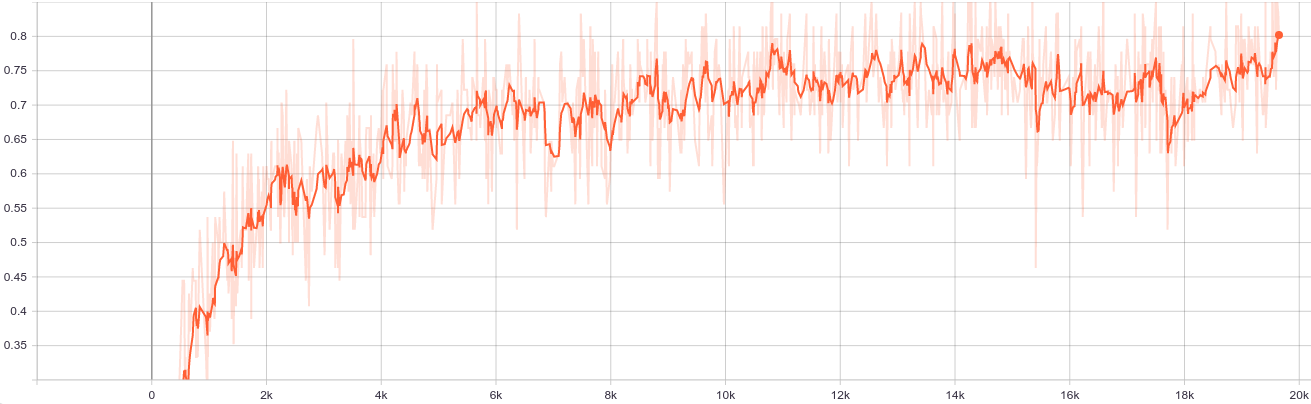
\includegraphics[width=\linewidth]{asset/image/first-result.png}
        \caption{Độ chính xác (acurracy) trên tập train sau các bước lặp}
        \label{fig:first-result}
    \end{center}
\end{figure}



